\chapter{Criptografía de clave pública}
\section{De la criptografía clásica a la de clave pública}
%TODO. Comentar algo de la historia que propició este cambio. Está en las transparencias.

\subsection{Enigma}
La máquina \textbf{enigma} funcionaba de acuerdo al siguiente esquema:
\begin{center}
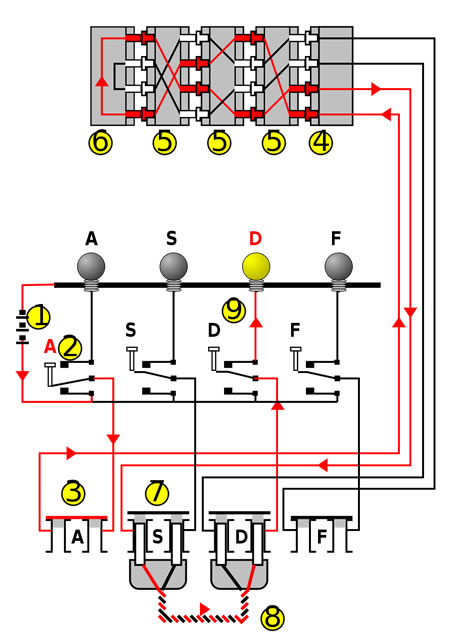
\includegraphics[width=0.6\textwidth]{img/enigma.jpg}
\end{center}
donde el número 8 representa uno de los modificadores, que simplemente conectaba pares de letras para que fuesen intercambiadas; el número 5 representa los rotores y el número 6 el reflector.

En rojo podemos ver el flujo que seguiría la corriente en caso de que pulsásemos la letra $A$, que sería cifrada a una $D$.

\obs La configuración que se muestra en la imagen sólo se mantendría fija durante un brevísimo periodo de tiempo. Tras finalizar el cifrado de la letra $A$, los rotores girarían de modo que no se volvería a seguir el mismo camino nunca más.

Si tenemos una máquina de enigma que funcione con 26 letras, 5 rotores de entre los que hay que escoger 3 y modificando 6 pares de letras\footnote{Es decir, tenemos 6 modificadores}, la pregunta que surge es clara, ¿Cuántas claves posibles tenemos?

Para empezar tenemos que escoger qué tres rotores tomamos, teniendo en cuenta que importa el orden, con lo que tenemos $5\cdot 4 \cdot 3 = 60$ opciones posibles.

Una vez hemos escogido los rotores, debemos ver qué posición tendrá cada rotor. Puesto que tenemos 26 posiciones para cada rotor tenemos un total de $26^3$ opciones.

Por último debemos colocar los modificadores, para lo que tenemos que elegir 6 pares de letras. Para ello tenemos un total de
\[{26 \choose 2} \cdot {24\choose 2}\cdot {22\choose 2}\cdot {20\choose 2}\cdot {18\choose 2}\cdot {16\choose 2} \text{ opciones }\]

Pero, puesto que no importa el orden, debemos dividir entre $6!$.

Agrupando todo lo que hemos mencionado, tenemos que la máquina \textbf{enigma} permite tener un total de:
\[\frac{60\cdot 26^3 \cdot {26 \choose 2} \cdot {24\choose 2}\cdot {22\choose 2}\cdot {20\choose 2}\cdot {18\choose 2}\cdot {16\choose 2}}{6!}\approx 8.469 \cdot 10^{17}  \text{ claves }\]

La forma de trabajar con \textbf{enigma} era mediante un libro de claves donde cada clave era empleada a lo largo de todo el día para todas las comunicaciones.

No obstante, si toda la flota empleaba el mismo sistema de cifrado y los mensajes eran fácilmente interceptables (se comunicaban por radio) al final sería relativamente sencillo que el enemigo descifrara la clave. Para solucionar esto, lo que se hacía es que al comienzo de cada mensaje se enviaban 3 letras, que indicaban la nueva posición de los rotores que debería emplearse a partir de ese momento.

Así, un esquema de transmisión del mensaje sería:
\begin{enumerate}
\item Montamos la máquina con la clave del día.
\item Transmitimos la clave del mensaje dos veces.
\item Cambiamos la posición de los rotores según la clave que enviamos.
\item Transmitimos el mensaje.
\end{enumerate}

Aquí tenemos la debilidad del criptosistema, el envío de la clave dos veces, puesto que nos adelanta cierta información acerca de la posición inicial de los rotores. Otro problema radicó en el hecho de que el primer mensaje del día siempre informaba del tiempo y siempre comenzaba de la misma forma, lo que daba aún más información a los enemigos.

A la hora de descifrar, el mecanismo es sencillo. La forma en que funciona \textbf{enigma} está basada en trasposiciones. Es decir, si a partir de la letra $A$ obtengo la $B$, a partir de la $B$ obtendré la $A$, partiendo de la misma clave.

Por tanto, una vez recibido el mensaje lo único que hay que hacer es introducir el mensaje cifrado en la máquina y como salida obtendremos el texto original.

Veamos por qué estos es cierto:
\begin{proof}
Para comprobar que la función de cifrado y su inversa son la misma, vamos a ver cómo funcionaba \textbf{enigma} sobre cada letra.

En primer lugar se intercambiaba una letra por otra mediante los modificadores. Tras esto la letra pasa por los rotores y llega al reflector (que será la clave de la demostración) y tras ello vuelve a pasar por los rotores y por el modificador.

Así nos queda que
\[\rho(m) = σ^{-1}δ^{1}Rδσ(m) \implies \rho^{-1}(m) = σ^{-1}δ^{1}Rδσ(m) = \rho(m)\]
\end{proof}

Pero ahora el lector avispado se percatará de un detalle muy importante. De todas las claves posibles que mencionamos al inicio de esta sección, no todas darán lugar a una función $\rho$ que coincida con su inversa.

En este caso, $\rho = \rho^{-1} \iff \rho = (a_1a_2)(a_3a_4)...(a_{25}a_{26})$, puesto que necesitamos que $\rho$ no haga más que permutar pares de letras.

Dada esta restricción tendremos un total de
\[\frac{{26 \choose 2} {24 \choose 2} ... {2 \choose 2}}{13!} =\frac{26!}{13!2^{13}} \approx 1.01 \cdot 10^{15} \text{ claves posibles }\]